\section{Message Brokers}

In the context of distributed systems, a message broker is an entity that coordinates the communication between a sender and a receiver. Message brokers are the core of Message Oriented Middleware. It enables the decoupling of sender and receiver by not having to keep the knowledge of each other \parencite{message_brokers}. It increases the modularity of an application. \ref{figures:message_broker} depicts the role of message broker, where it acts as co-ordinator between the publishers and subscribers.

\makeatletter
\setlength{\intextsep}{25pt}
\makeatother

\begin{figure}[h]
\centering
\includegraphics[keepaspectratio, width=.7\textwidth, trim={0 10cm 0 8cm},clip]{message_broker.eps}
\caption{Message Broker}\label{figures:message_broker}
\end{figure}

While the primary function of a message broker is to decouple a sender and receiver, it can also perform other activities \parencite{message_brokers_usage} such as:

\begin{itemize}
  \item Messaging routing to one or more destinations
  \item Message transformation to an alternative representation
  \item Aggregating messages and delivering them to the receiver. Further receiving acknowledgments and composing them into a single response to deliver back to the sender.
  \item Routing messages in content and topic-based publish-subscribe pattern
  \item Provides guarantees regarding message delivery and transaction management.
\end{itemize}